\chapter[Characterization]{Characterization of Pulsars and Sub-Luminous Populations}
\label{chapter:collaborationWork}

This chapter focuses on work done in collaborations with others.
Main contributions are in modeling polarization position angle data
using the rotating vector model (RVM) and the numerical model. 
Example work will include use
of the models 
for general characterization of pulsars
and for a population study of $\gamma$-ray sub-luminous pulsars.
Because of the collaborative nature of the
work, this chapter will also focus on the broader use of polarization
data in conjunction with other types of data.
For the most part, $\gamma$-ray
modeling was performed by Roger W. Romani.

First, We will discuss the paper ``PSRs J$0248+6021$ and J$2240+5832$: Young Pulsars 
in the Northern Galactic Plane. Discovery, Timing, and Gamma-ray observations''
\citep{theureau2011psrs} in which two pulsars are reported as detected in the $\gamma$-ray
by the {\it Fermi} Large Area Telescope.  Many properties of the pulsars are characterized
using $\gamma$-ray and radio data.

PSR J1119-6127 is likewise characterized in ``Observations of Energetic High Magnetic Field Pulsars with the
{\it Fermi} Large Area Telescope'' \citep{parent2011observations}.  
A number of high magnetic field pulsars are discussed in the paper and PSR J1119-6127
is analyzed with a single-altitude polarization model.

In ``Broad-Band KeV to MeV Characteristics Of Soft Gamma-Ray Pulsar PSR J1513$-$5908''
\citep{hartogJ1513}, the pulsar PSR J1513$-$5908 (B1509$-$58) is analyzed in a 
number of wavelengths using revisited and updated data.  We analyze the
radio polarization using a single-altitude model.

The pulsar PSR J0737$-$3039A is analyzed using a two-altitude 
polarization model in ``{\it Fermi} LAT Pulsed
Detection of PSR J0737$-$3039A in the Double Pulsar System''.
We also include scattering effects in this model although it 
is difficult to reproduce the scattering effects seen in the data.  
This pulsar has complex polarization, which we selectively
cut.  This pulsar is particularly interesting because few
mildly spun-up pulsars have been detected in the $\gamma$-rays.

Finally, We will discuss the paper ``Sub-luminous $\gamma$-Ray Pulsars''
\citep{romani2011sub}.  The paper examines a number of young radio pulsars
that are weak in the $\gamma$-rays.  We try to determine
whether this sub-luminosity is due to
aligned geometry
using geometric constraints 
(including six pulsars for which we perform analysis using radio polarization).


\section{PSR J0248$+$6021 and PSR J2240$+$5832: Characterizing Young Pulsars with RVM}
\paperref{This section is based on work done for
``PSRs J0248$+$6021 and J2240$+$5832: Young Pulsars in the Northern Galactic
Plane. Discovery, Timing, and $\gamma$-Ray Observations''
\citep{theureau2011psrs}. }


\begin{figure}[t!!]
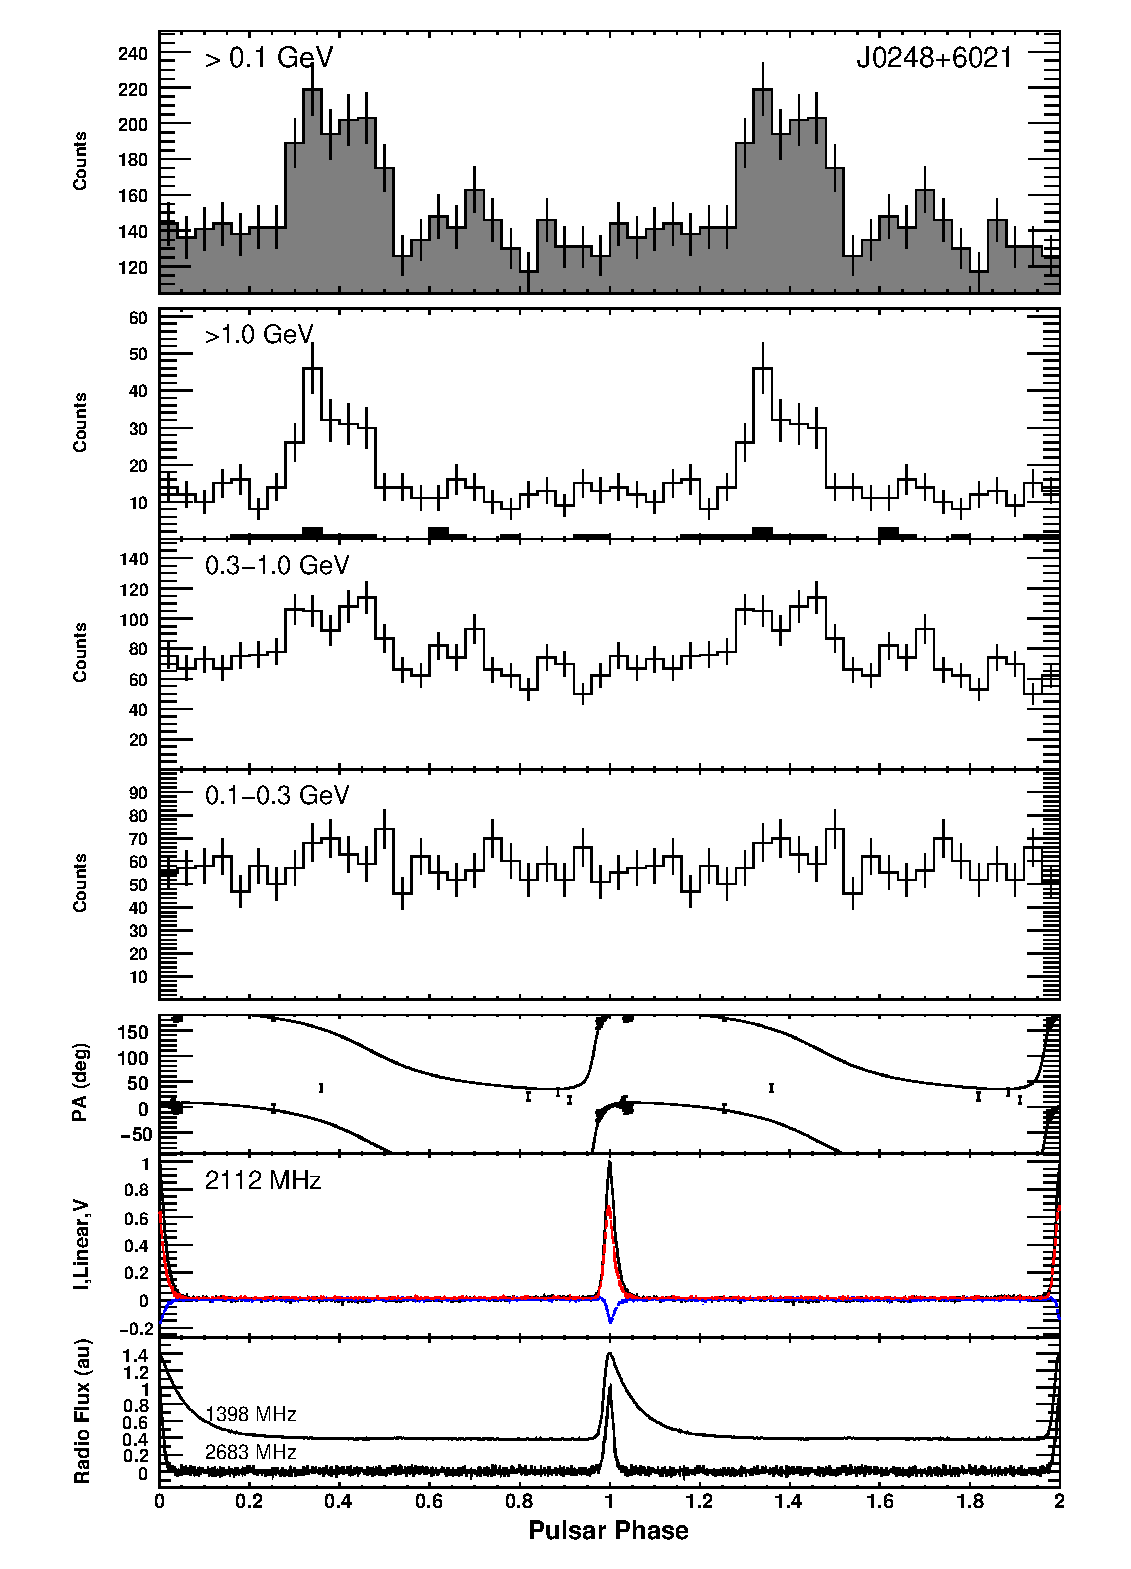
\includegraphics[width=0.5\textwidth]{chapters/multiWaveLength/figures/J0248+6021_catalog_lightcurve.eps}
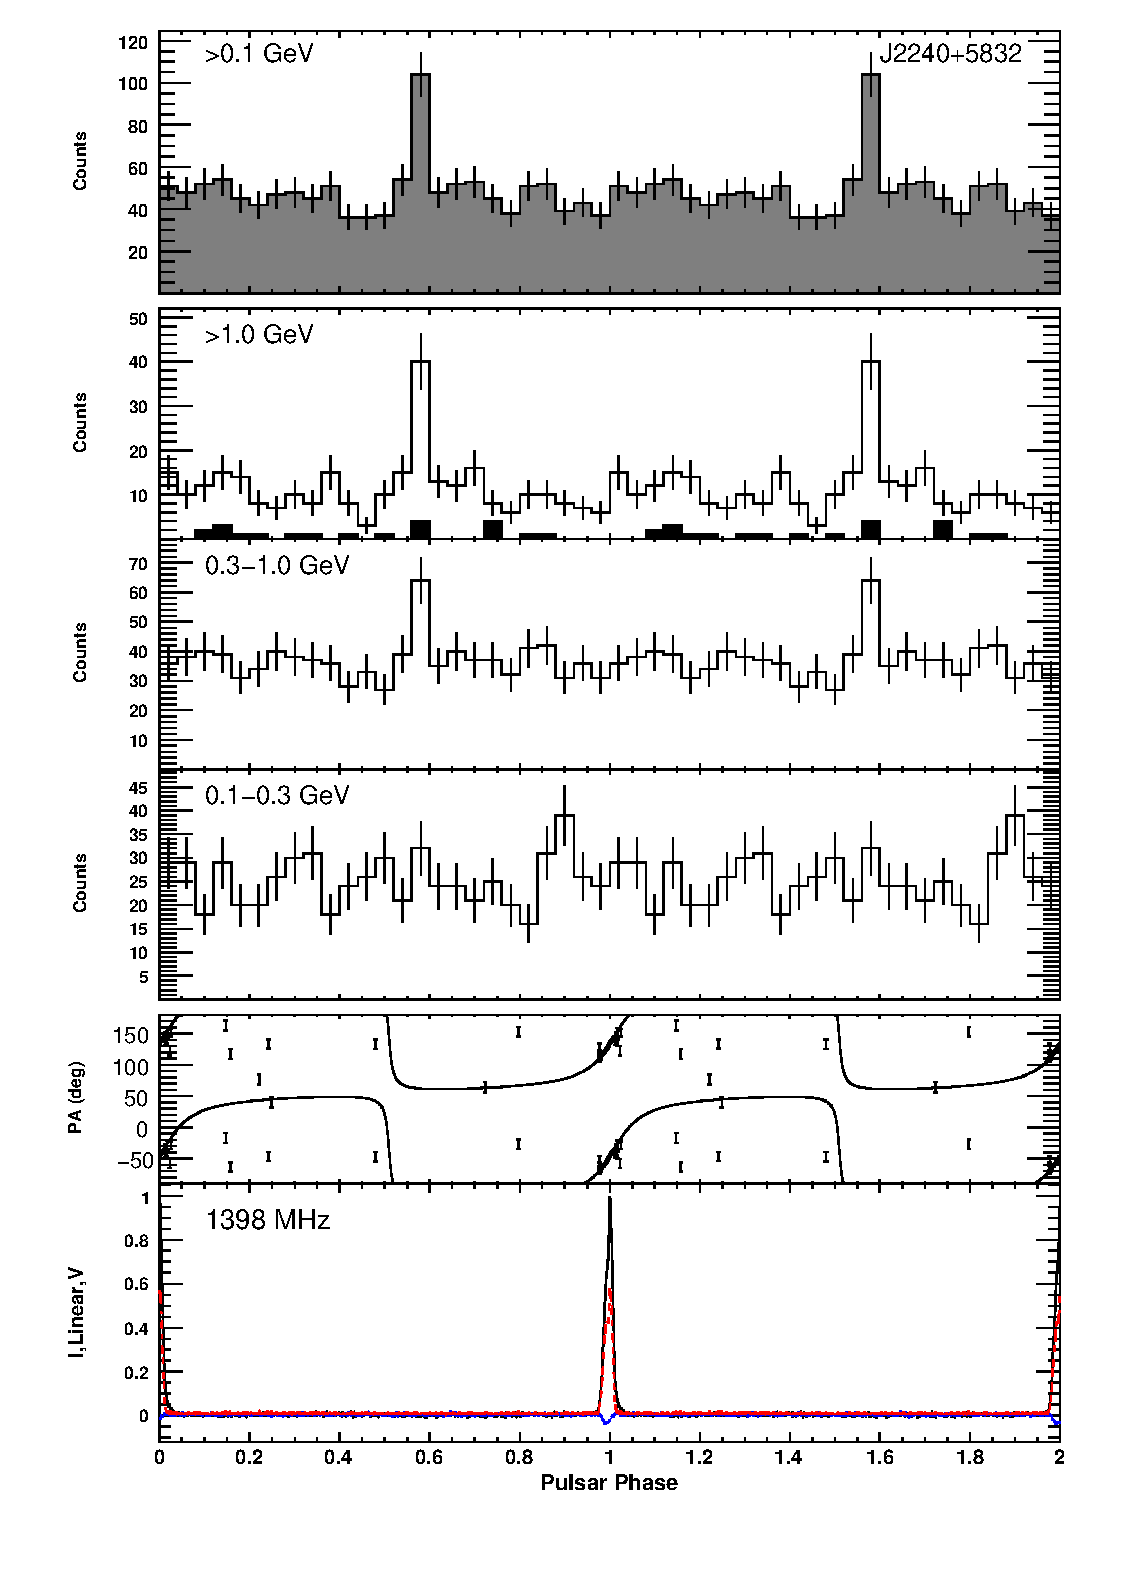
\includegraphics[width=0.5\textwidth]{chapters/multiWaveLength/figures/J2240+5832_catalog_lightcurve.eps}
\caption[Phase-aligned $\gamma$-ray and radio light curves for PSR J0248$+$6021 and PSR J2240$+$5832 obtained with
the \emph{Fermi} Large Area Telescope and the Nan\c cay Radio Telescope]{
Figure taken from \cite{theureau2011psrs}.
Phase-aligned $\gamma$-ray and radio light curves for PSR J0248$+$6021 and PSR J2240$+$5832 obtained with 
the \emph{Fermi} Large Area Telescope and the Nan\c cay Radio Telescope. 
The bottom panel for PSR J0248$+$6021 show the radio profiles at three frequencies. 
The second panel from the bottom
for PSR J0248$+$6021 and the bottom panel for PSR J2240$+$5832 
show the degree of linear (red dashed) and circular
polarizations (blue dotted), as well as the linear polarization position angle and a RVM fit.
The other panels show the
$\gamma$-ray light curve data in different energy bands. Two rotations are shown for clarity.}
\label{phasos}
\end{figure}

\begin{figure}[t!!]
\begin{center}
\includegraphics[width=0.8\textwidth]{chapters/multiWaveLength/figures/J0244Alpha46Zeta52Offset2.53133ANDJ2238Alpha108Zeta123Offsetneg45.818.ps}
\caption[Expanded view of the radio polarization position angle sweep near the peak in radio intensity]{Figure taken from \cite{theureau2011psrs}.
Expanded view of the radio polarization position angle sweep near the peak in radio intensity. 
The red points show the data used in the RVM fit. The black points failed the selection cuts
described in the text. Top two frames are data for PSR J2240$+$5832 at 1.4 GHz. The RVM curve shown corresponds to $\alpha = 108^\circ$ and $\zeta = 123^\circ$. Bottom two frames are data for PSR J0248+6021
at 2.1 GHz. The RVM curve shown corresponds to $\alpha = 46^\circ$ and $\zeta =52^\circ$.  \label{PolarZoom}
}
\end{center}
\end{figure}

\begin{figure}[t!!]
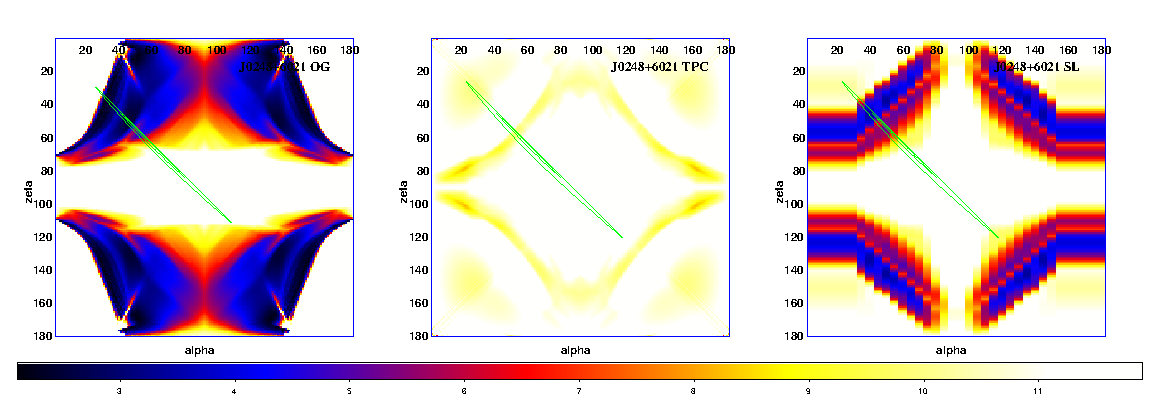
\includegraphics[width=1\textwidth]{chapters/multiWaveLength/figures/New_J0248_OGTPCSL.eps}
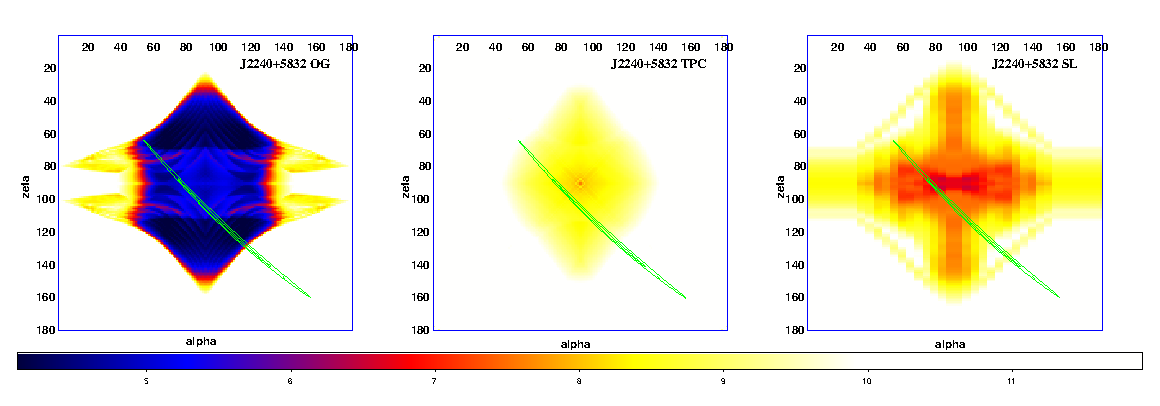
\includegraphics[width=1\textwidth]{chapters/multiWaveLength/figures/New_J2240_OGTPCSL.eps}
\caption[Pulsar geometry and emission modeling fit map for PSR J0248$+$6021 and PSR J2240$+$5832 in the $\alpha$--$\zeta$ plane]{Figure taken from \cite{theureau2011psrs}.
Pulsar geometry and emission modeling fit map for PSR J0248$+$6021 and PSR J2240$+$5832
in the $\alpha$--$\zeta$ plane. Green 
contours show the RVM fit to the radio polarization data. 
Contours are at $\delta(\chi^2/\text{Degree of Freedom}) = 0.25$ and $0.5$ above the minimum $\chi^2/\text{Degree of Freedom}$ of 1.6
for PSR J0248$+$6021 and $\delta(\chi^2/\text{Degree of Freedom}) = 0.4$ and $0.8$ above the minimum $\chi^2/\text{Degree of Freedom}$ of 5.1
for PSR J2240$+$5832.
The color backgrounds are $\chi_3$ maps of the fit to the observed $>100$\,MeV
pulse profile for the outer gap model (left),
the two-pole caustic model (middle), and the separatrix layer model (right), 
at different values of the magnetic inclination,
$\alpha$, and the minimum angle to the line-of-sight, $\zeta$ \citep{romani2010constraining}.
Each panel has the same color scale, where dark colors represent better fits. The
preferred models lie along the green RVM-selected band.
}
\label{OGTPC}
\end{figure}


PSR J0248$+$6021 ($P=217$ ms) and PSR J2240$+$5832 ($P=140$ms) are young pulsars first discovered in the radio
\citep{foster1997fast,ray1999j0248+}.  The polarization sweep for both pulsars is relatively smooth
such that likely only a single-altitude component contributes to the emission.

For these two pulsars, we applied both the RVM and $\gamma$-ray light curve models
to the available data.
Figure~\ref{phasos} shows the light curves at various wavelengths
as well as the polarization data.
Modeling results indicate that the $\gamma$-ray emission from PSR J0248$+$6021
is from a merged double $\gamma$-ray peak while the emission from 
PSR J2240$+$5832 is from a narrow caustic.
The paper discusses various measurements of the
pulsars PSR J0248$+$6021 and PSR J2240$+$5832 such as
flux density, proper motion, dispersion measure, kick velocity, and rotation
measure. 

We applied the RVM to the polarization data of 
PSR J0248$+$6021 (2.1 GHz) and PSR J2240$+$5832 (1.4 GHz).  
We cut on polarization with error bars greater than
 $\pm 2^\circ$.
The polarization position angle sweeps are flattened
due to scattering.  Data at 1.4 GHz was avaliable for PSR J0248$+$6021
but appeared distorted by scatter so only the 2.1 GHz data was used.
Red error bars on Figure~\ref{PolarZoom} show points
used in the fitting procedure.  

For PSR J0248$+$6021, the best fits give geometric angles $\beta\sim5^\circ$ 
(where $\beta=\zeta-\alpha$) and $\alpha$ between $25^\circ$ and $110^\circ$.
The best $\chi^2$ is 86.6 with reduced $\chi_{\rm{min}}^2=1.6$.
For PSR J2240$+$5832, the best fits give geometric angles $\beta\sim16^\circ$ and $\alpha$ between $75^\circ$ and $130^\circ$
although plausible solutions extended to $\alpha$ between $10^\circ$ and $150^\circ$.
The best $\chi^2$ is 86.6 with reduced $\chi_{\rm{min}}^2=1.6$.
Figure~\ref{PolarZoom} additionally shows reasonable model polarization sweeps
overlaid on data points.

On Figure~\ref{OGTPC}, green contours trace the best fit RVM in the $\alpha$-$\zeta$ plane.
The colored maps show best fit outer gap model, two-pole caustic model, 
and separatrix layer model \citep{bai2010modeling} to the $\gamma$-ray data.
The weighting used is the $\chi_3$ of \cite{romani2010constraining}.
For PSR J0248$+$6021, the best fit overlap between outer gap and RVM
model is $\alpha=46^\circ$ and $\zeta=52^\circ$.
For PSR J2240$+$5832, the best fit overlap between outer gap and RVM
models is $\alpha=101^\circ$ and $\zeta=117^\circ$.
Overall, the outer gap model seemed to be more consistent
with the polarization model results
than the other $\gamma$-ray models.





\section{PSR J1119$-$6127: Characterization a High Magnetic Field Pulsar with Single-Altitude Model}

\paperref{This section is based on work done for
``Observations of Energetic High Magnetic Field Pulsars with the
\it{Fermi} Large Area Telescope'' \citep{parent2011observations}.}

\begin{figure}[t!!]
%\begin{center}
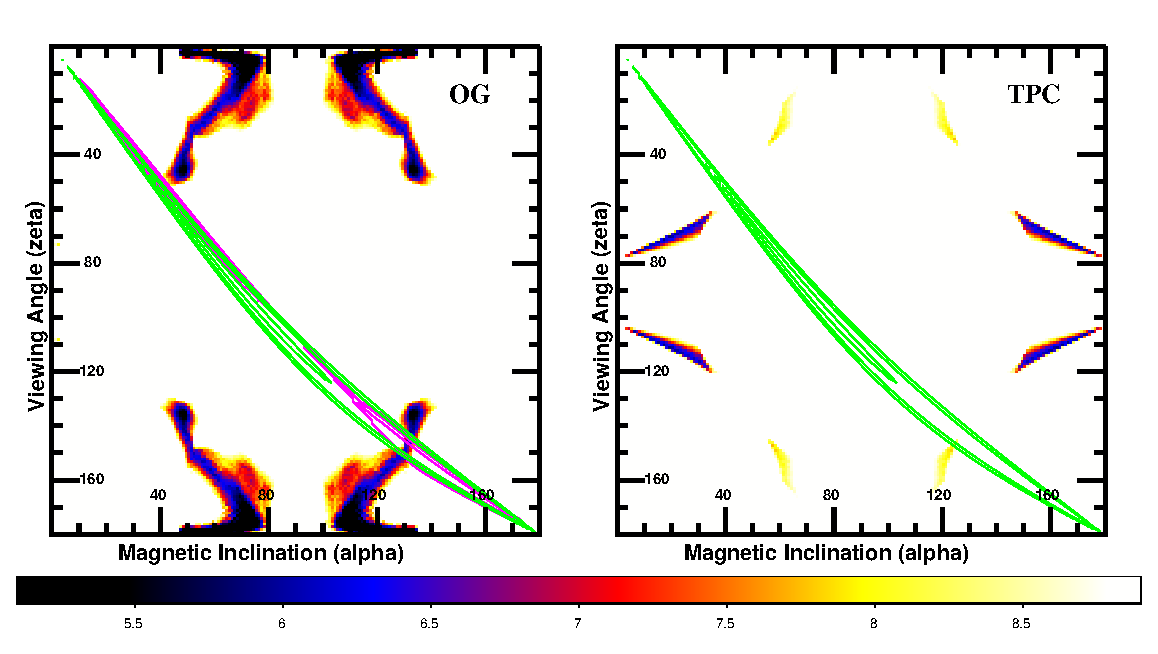
\includegraphics[width=0.99\textwidth]{chapters/multiWaveLength/figures/HBP_fig3_rev.eps}
\caption[Pulsar geometry and emission modeling fit map for PSR~J1119$-$6127 with the outer gap
(left panel) and the two-pole caustic (right panel) models in the $\alpha$--$\zeta$ plane]{
Figure taken from \cite{parent2011observations}.
Pulsar geometry and emission modeling fit map for PSR~J1119$-$6127 with the outer gap
(left panel) and the two-pole caustic (right panel) models in the $\alpha$--$\zeta$ plane. Green contours show
the RVM fit to the \cite{weltevrede2011glitch} radio polarization data. For
the left panel we also show the polarization fit for finite-altitude, open zone
radio emission ($R=0.09\,R_{\rm{LC}}$, magenta contours). Contours are at
1.5, 2.5, and 3.5 times the minimum value of the reduced
$\chi^2 = 0.85$. The background color scale gives the $\chi_3$ statistic fit to
the observed $> 500$\,MeV $\gamma$-ray pulse profile. The color scales in the panels are the
same, with dark colors representing better fits. Preferred models lie along the
diagonal polarization fit band. \label{fig:roger_goodness}}
%\end{center}
\end{figure}

\begin{figure}
\begin{center}
\includegraphics[scale=0.75]{chapters/multiWaveLength/figures/HBP_fig4_rev.eps}
\caption[Light curves and radio polarization of PSR~J1119$-$6127 overlaid with models]{
Figure taken from \cite{parent2011observations}.
Light curves and polarization of PSR~J1119$-$6127 overlaid with models. The bottom panel shows the Parkes
radio light curve in the two peaked (post-glitch) mode, which provides the best
model constraints. The corresponding radio polarization position angle data are
shown (right scale) in the upper panel. The model pulsar phase ($\phi_{\rm{B}}$, bottom axis) is
referenced to the closest approach of the magnetic axis to the Earth
line-of-sight, as fit from the polarization sweep. The sweep rate maximum
(green arrow) and pulse profile offsets (magenta arrow) are shown, with good
matches to the observed radio data for an altitude of $R=0.09 R_{\rm{LC}}$. The
upper panel shows the {\it Fermi} pulse profile (left scale) and model outer gap (solid line)
and two-pole caustic (dashed line) profiles. These are best-fit profiles (geometric angles
in the legend) and the phase is referenced to the radio-determined phase of the
magnetic axis. The $\gamma$-ray background, shown by the dotted line, was
estimated using an annular ring centered on the radio position with inner and
outer radii of 0.5\degr\ and 1.5\degr\ respectively, during the off-pulse
region. \label{fig:roger_lcs} } \end{center}
\end{figure}

In the paper \cite{parent2011observations}, detection 
with the {\it Fermi} Large Area Telescope
of PSR J1119-6127 (Period $=0.408s$) and 
upper limits of pulsars PSR J1718-3718, PSR J1734-3333 and PSR J1846-0258
are reported and criteria for non-detection are discussed.
These pulsars have high magnetic fields.
In the paper, the spectrum of PSR J1119-6127 is concluded to be more 
similar to a young pulsar rather than a magnetar as might
be expected from such a high magnetic field.

Data used to analyze the radio polarization was
taken during a 
glitch recovery in PSR J1119-6127 wherein
more data per phase was available.
Because of the larger number of avaliable data points,
modeling the polarization position
angles was more constraining.
Data analysis details are given in 
\cite{weltevrede2010pulsar} and \cite{hobbs2004long}.

In the $\gamma$-ray modeling, both two-pole caustic
and outer gap models were tested with
$w=0.02$.  Results of these fittings are seen in 
Figure~\ref{fig:roger_goodness}. 
The figure of merit here is the  
$\chi_3$ weighting defined in \cite{romani2010constraining}.
Additionally, on the plot are the  
RVM fit contour results in green as well as a numerical 
single-altitude model fit contour in magenta.  
Two-pole caustic fitting results and the polarization
fitting results have poor overlap compared to the outer gap model.
The best models are at $\alpha=125^\circ$ to $130^\circ$
and $\zeta=140^\circ$ to $150^\circ$ for the outer
gap model and at $\alpha=125^\circ$ and $\zeta=145^\circ$
for the two-pole caustic model. 
The two models give similar geometry angles but 
the outer gap model is a better
fit over a larger parameter space as can be seen in Figure~\ref{fig:roger_lcs}

The best fit parameters for polarization
modeling yield reduced $\chi^2$ of 1.1
The altitude of emission derived
from polarization fitting is $0.1R_{\rm{LC}}$.
It is interesting to note that 
using the BCW model yields lower altitudes 
\citep{weltevrede2011glitch} and requires smaller
$\alpha$ for emission originating in the open zone.




\section{PSR J1513$-$5908: Characterizing a Soft $\gamma$-ray Pulsar with Single-Altitude Model}
\paperref{
This section is based on work done for
``Broad-Band KeV to MeV Characteristics of Soft $\gamma$-Ray Pulsar PSR J1513$-$5908''
\citep{hartogJ1513}.}

\begin{figure}[htbp]
\begin{center}
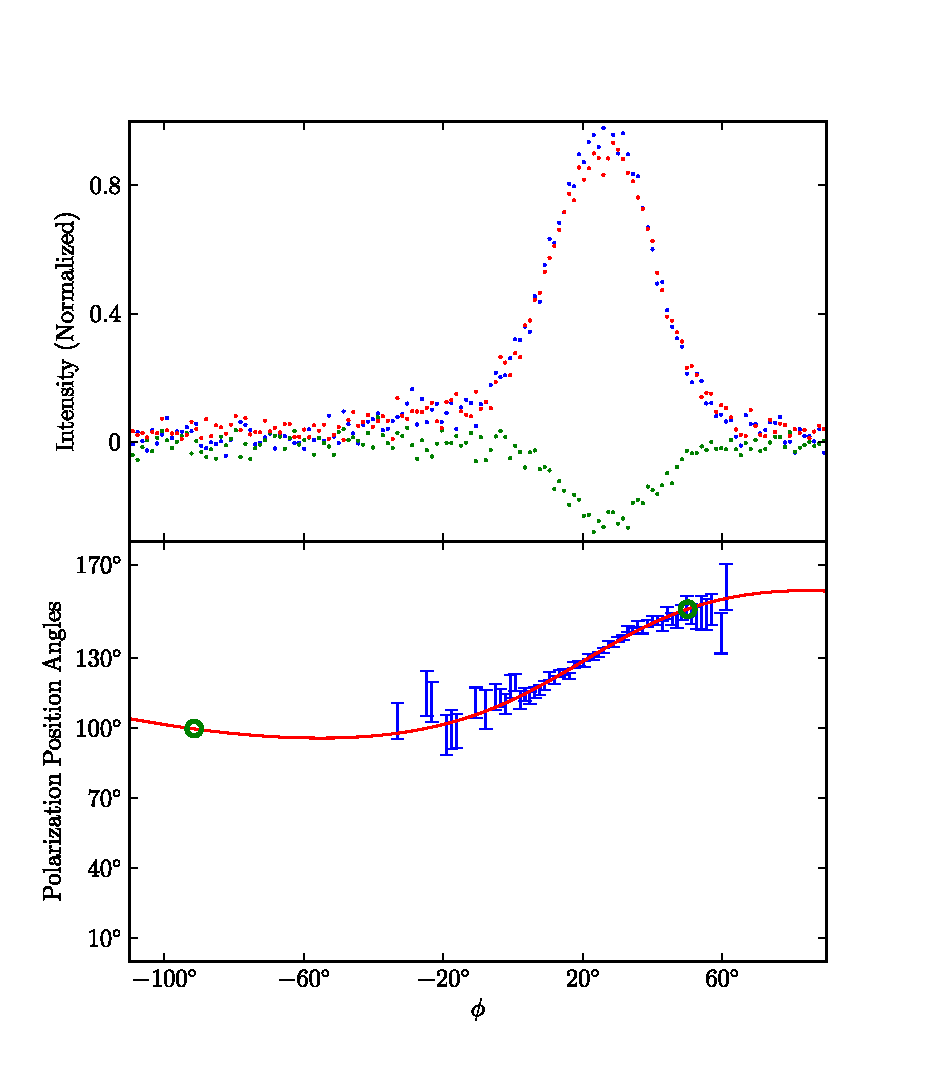
\includegraphics[scale=.8]{chapters/multiWaveLength/figures/intAndPAJ1513alpha153zeta133.eps}
\caption[Intensity and polarization data for PSR J1513$-$5908 overlaid with model]{\label{fig:intAndPAJ1513alpha153zeta133}
Figure taken from \cite{hartogJ1513}.
Intensity and polarization data for PSR J1513$-$5908 overlaid with model.
In the upper panel, blue points are total intensity data, red points are linear polarization intensity data,
and green points are circular polarization intensity data for PSR J1513$-$5908 at 20 cm.
In the bottom panel, blue error bars are polarization position angles
used in the fit. 
The red solid line is the fit model
polarization with $R=0.24R_{\rm{LC}}$, $\alpha=153^{\circ}$, and $\zeta=133^{\circ}$. 
Empty circles mark phase of emission from open field lines.
}
\end{center}
\vskip -0.2truecm
\end{figure}

\begin{figure}[t!!]
\begin{center}
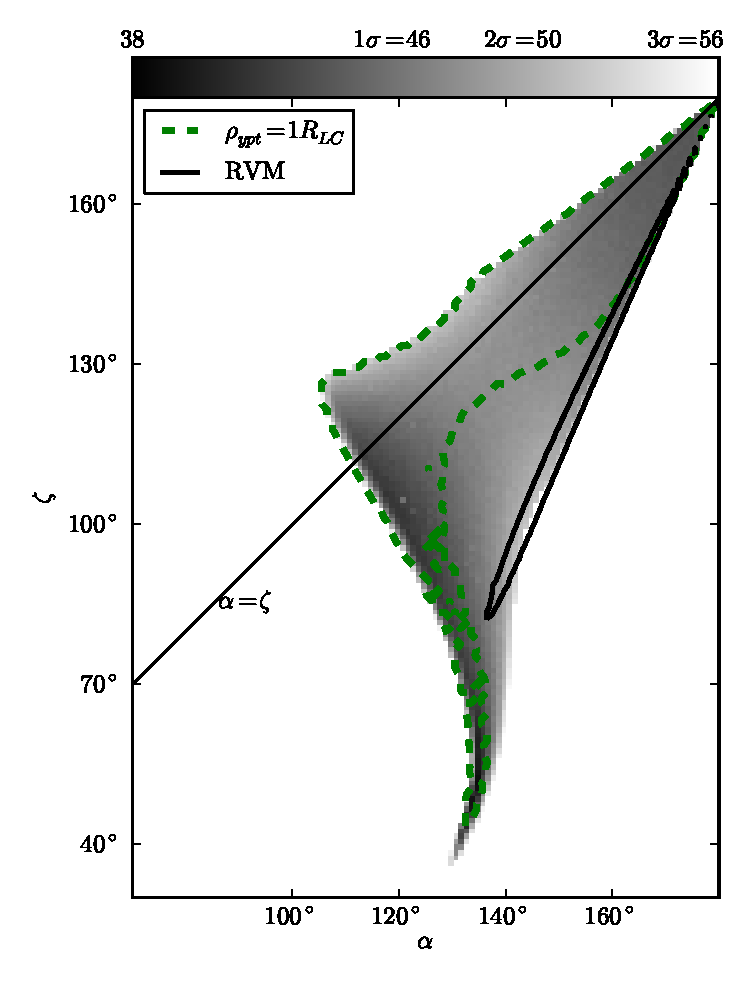
\includegraphics[scale=.8]{chapters/multiWaveLength/figures/J1513-5908Map.eps}
\caption[Map of $\chi^{2}$ for PSR J1513-5908 fit to radio polarization in the $\alpha$-$\zeta$ plane]{\label{fig:J1513-5908Map}Figure taken from \cite{hartogJ1513}.
Map of $\chi^{2}$ for PSR J1513-5908 fit to radio polarization in the $\alpha$-$\zeta$ plane.
Overlaid are  $3\sigma$ above $\chi^2_{\rm min}$ contour for
zero altitude RVM fit (black) and $3\sigma$ above $\chi^2_{\rm min}$ contour for the assumption that emission must come from the formal open
zone.
}
\end{center}
\vskip -0.2truecm
\end{figure}

\begin{figure}[htbp]
\begin{center}
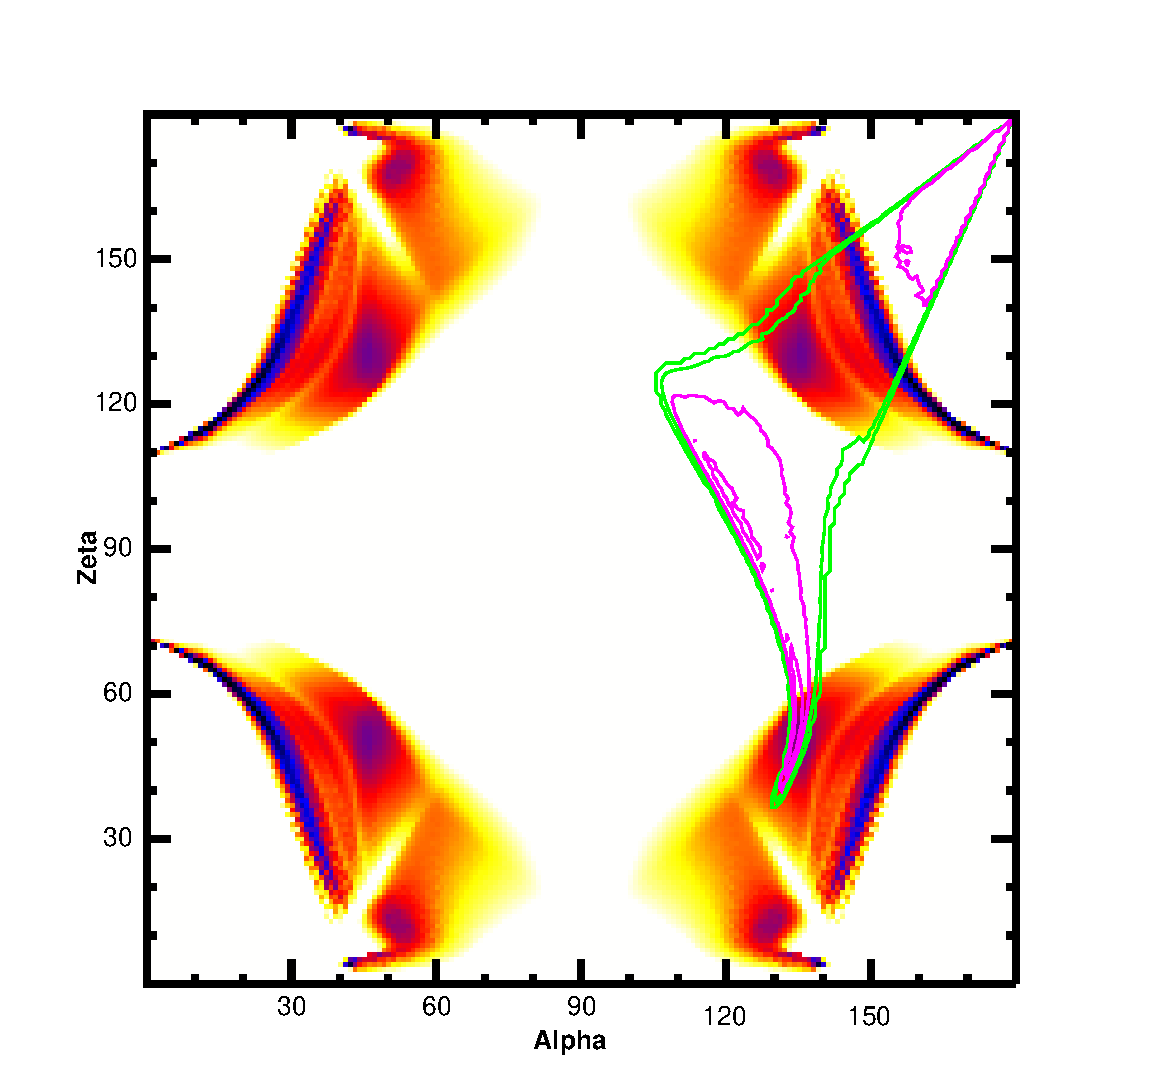
\includegraphics[scale=.8]{chapters/multiWaveLength/figures/BJ1513_w10.eps}
\caption[Pulsar geometry and emission modeling fit map of an outer gap model and radio polarization model 
for PSR J1513$-$5908 in
the $\alpha$--$\zeta$ plane of the pulsar]{\label{fig:BJ1513_w10}
Figure taken from \cite{hartogJ1513}.
Pulsar geometry and emission modeling fit map of an outer gap model 
and radio polarization model for PSR J1513$-$5908 in
the $\alpha$--$\zeta$ plane. Contours show the polarization
fit of the $0.5\sigma$ and $1.0\sigma$ regions in magenta;
and the $2.0\sigma$ and $3.0\sigma$ regions in green.
A wide range of geometries is allowed by these polarization data,
including the best $\gamma$-ray fits. Good fits must also match the
phase of the magnetic dipole axis (see text).
}
\end{center}
\vskip -0.2truecm
\end{figure}

\begin{figure}[htbp]
\begin{center}
\includegraphics[width=\textwidth]{chapters/multiWaveLength/figures/J1513_lc.eps}
\caption[Radio and $\gamma$-ray light curves of PSR J1513$-$5908 with model light curve for $\alpha=153^\circ$, $\zeta=133^\circ$]{\label{fig:J1513_lc}
Figure taken from \cite{hartogJ1513}.
Radio and $\gamma$-ray light curves of PSR J1513$-$5908 with model light curve for $\alpha=153^\circ$, $\zeta=133^\circ$.
A single
peak dominates since the line of sight skims the $\gamma$-ray caustic. The
radio emission altitude is 0.24$R_{\rm LC}$ and polarization and
$\gamma$-ray fits both indicate that the magnetic axis (green upwards arrow)
leads the radio peak by $\phi=0.08$.
}
\end{center}
\vskip -0.2truecm
\end{figure}



The paper ``Broad-Band KeV to MeV Characteristics of Soft $\gamma$-Ray Pulsar PSR J1513$-$5908''
\citep{hartogJ1513} aims to do a 
spectral study covering 2 KeV to 1 GeV including 
updated {\it Fermi} data and revisited archival RXTE-PCA and HEXTE data
along with historic CGRO-COMPTEL data of the pulsar PSR J1513$-$5908 (PSR B1509$-$58).
The pulsar was also analyzed using radio polarization data.

The polarization data analyzed is 1.4 GHz data.
The pulsar PSR J1513$-$5908 has a period of 151 ms.
Also noted in the paper is
an extra component in the radio intensity of PSR J1513$-$5908
before the peak of the main pulse.
We had hoped to model this component using polarization
but the scatter of the data was too large to derive
useful fit results.

The typical retarded dipole with photons projected tangent to the magnetic
field lines is used to calculate the position 
angles of the polarization.  Further, models used here
extrapolate from the classical RVM allowing emission from finite
radial altitudes above the surface of the neutron star with relativistic and sweep-back effects.  
Allowed altitudes ranged between
$.002R_{\rm{LC}}$ (the radius of the neutron star assuming $R_{\rm{NS}}\sim 15$ km) to $.9R_{\rm{LC}}$.

Figure~\ref{fig:intAndPAJ1513alpha153zeta133} shows the polarization position angle sweep and intensity
profile for 20 cm data.  The sweep is relatively simple and shows no signs of orthogonal
mode jumps or multiple altitude.  RVM fits relatively well to the polarization with
$\chi^2_{\rm{min}}=44$ for Degree of Freedom=DOF$=55-4$.  The four fit parameters are $\alpha$, the angle between
the magnetic axis and rotation axis, $\zeta$, the viewing angle as measured from the rotation
axis and the horizontal and the vertical offsets in the 
polarization angles.  The best fit model
with finite altitude has $\chi^2_{\rm{min}}=39$ for DOF$=55-5$ although the best fit model might
not be the most physically viable model as will be discussed later.  The solid red line in
Figure~\ref{fig:intAndPAJ1513alpha153zeta133} is a finite-altitude model at $\alpha=153^\circ$,
$\zeta=133^\circ$, and $R=0.24R_{\rm{LC}}$ with $\chi^2=48$.  Green circles on the
solid red line mark the expected end of emission based on a formal open zone assumption.


Figure~\ref{fig:J1513-5908Map} shows the best fit $\chi^2$ surface map projection in the
$\alpha$-$\zeta$ plane for the single-altitude model.  
The $3\sigma$ contours for the RVM fit are
overlaid on the color map in black.  Additionally, on this panel is a green contour that
encloses the model parameters for which model emission phase is equal to or greater than
the emission phase seen in the data.  The model emission phase is defined by the emission
from the classic open field lines.  Overlap between these contours is minimal.  This indicates
a physical need to increase emission phase from RVM either by increasing the altitude of emission
or widen the open zone cap.

Following \cite{romani2010constraining} we fit the $\gamma$-ray
light curve using the $\chi_3$ statistic. While PSR J1513$-$5958 is
very energetic, implying a small gap and emission close to the last closed
field lines, we find appreciably better light curves for a modest gap width,
$w=0.05-0.1$. In Figure~\ref{fig:BJ1513_w10}, the background color scale shows the goodness of
fit for an outer gap  model with $w=0.1$. Overlaid are
contours from the radio fitting. To be a viable model, the $\gamma$-ray fit
must lie inside the radio contours. Since the polarization presents a simple sweep, this
is not very constraining, with a wide range of geometries compatible at the
$3\sigma$ level. However, the polarization fit also tightly constrains
the phase of the magnetic axis relative to the radio intensity peak. For
a viable model, this should match as well.

The strip of best $\gamma$-ray fits crosses the radio-allowed region
along $\alpha=153^\circ$ and $\zeta=145^\circ$ to 
$\alpha=156^\circ$ and $\zeta=128^\circ$
with $\chi_3<4.5$. In
this region the phase of the magnetic axis ranges from $-0.06$ to $-0.08$
(in fractions of a period)
and the radio emission altitude varies from $0.1$ to $0.3R_{\rm LC}$.
In Figure~\ref{fig:J1513_lc}, we show the fit $\gamma$-ray light curve 
for $\alpha=153^\circ$ and $\zeta=133^\circ$.
The radio fit altitude is $0.24R_{\rm LC}$ and the polarization
fit is $1.2\sigma$ from its minimum. In this region {\it both}
the $\gamma$-ray and polarization fits place the magnetic dipole axis
0.08 before the radio peak.  A second region of plausible $\gamma$-ray fits
(with $\chi_3 \approx 5.4$) lies close to the polarization fit minimum.
In this region, $\alpha=135^\circ$ and $\zeta=51^\circ$ 
and the $\gamma$-ray light curve, while
dominated by a single peak, has a tail to phase $0.5$.  However the fit magnetic
axis phases do not agree (-0.03 for $\gamma$-ray, 0 for radio) and the radio
altitude is quite high, 0.75 to 0.85$R_{\rm LC}$. At this altitude the details
of the magnetic structure are less reliable; so we prefer the lower altitude
solution with the correct phase match. At this lower altitude, there is
also room for the field lines to open within the light cylinder, giving
a y-point radius $<1$ and a larger effective $w$.


\section{PSR J0737$-$3039A: Characterizing a Double Pulsar System with Finite-Altitude Model}
\paperref{This section is based on work done for ``\it{Fermi} LAT Pulsed
Detection of PSR J0737$-$3039A in the Double Pulsar System'' \citep{guillemot2013fermi}.}

\begin{figure*}[t!!]
\begin{center}
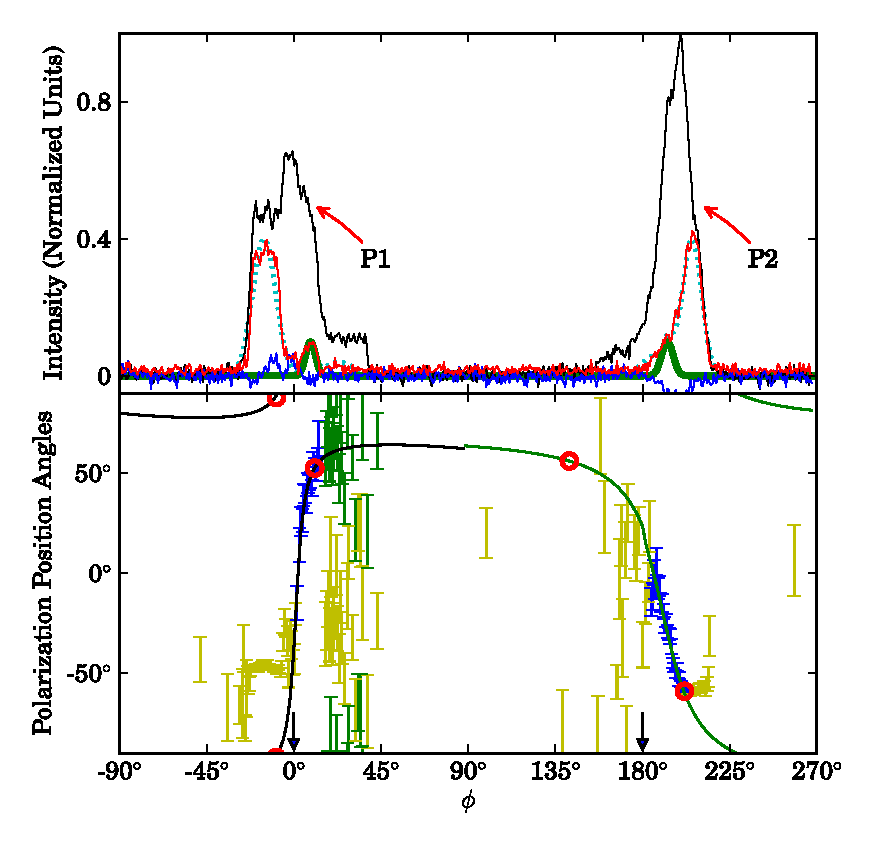
\includegraphics[width=0.9\textwidth]{chapters/multiWaveLength/figures/figure3-0737.eps}
\caption[Polarimetric profile for PSR J$0737-3039$A as observed at 1.4 GHz
with the Parkes radio telescope]{
Figure taken from \cite{guillemot2013fermi}.
Polarimetric profile for PSR J$0737-3039$A as observed at 1.4 GHz
with the Parkes radio telescope (R.~N.~Manchester, private communication). Top panel:
Stokes parameter curves (black is total intensity, red is linear polarized intensity, and
blue is circularly polarized intensity) and Gaussian decomposition
of the linear intensity components (dotted curve is all linear and the thick green
curve gives the rapid sweep central component fit here). Bottom: position angle
data (blue: central components, yellow: other position angle values, green: P1 tail with
an orthogonal mode jump). The smooth curves give the best fit model for the two
poles while the red circles denote the boundaries of the open zone at the
emission altitude. Arrows denote the phase of the closest approach of the
magnetic axes to the Earth line-of-sight.
\label{fig:polarfit}} \end{center}
\vskip -.3truecm
\end{figure*}


\begin{figure*}[t!!]
\begin{center}
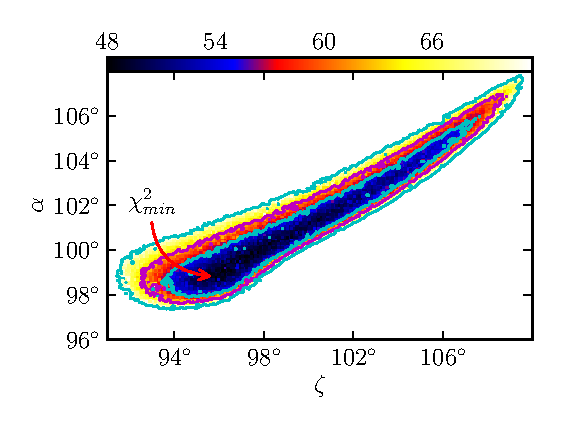
\includegraphics[width=0.9\textwidth]{chapters/multiWaveLength/figures/figure4-0737.eps}
\caption[Map of $\chi^2$ surface of the RVM fit to the radio polarization data
(central components) for PSR J$0737-3039$A in the $\alpha$--$\zeta$
plane]{Figure taken from \cite{guillemot2013fermi}. Map of $\chi^2$
surface of the RVM fit to the radio polarization data (central components) for
PSR J$0737-3039$A in the $\alpha$--$\zeta$ plane. The best fit orientation
angles ($\alpha,\, \zeta$) are indicated by an arrow, while the contours are
shown at the $1\sigma$, $2\sigma$ and $3\sigma$ levels above $\chi^2_{\rm min}$.\label{fig:polarchisq}}
\end{center}
\vskip -.3truecm
\end{figure*}


\begin{figure*}[htbp]
\begin{center}
\includegraphics[width=0.9\textwidth]{chapters/multiWaveLength/figures/figure5-0737.eps}
\caption[Light curves for PSR J$0737-3039$A at the $\alpha$ and $\zeta$ angles determined 
from the radio polarization study]{Figure taken from \cite{guillemot2013fermi}.
Light curves for PSR J$0737-3039$A at the $\alpha$ and $\zeta$ angles determined
from the radio polarization study, and for the outer gap model (solid blue line) and the
two-pole caustic model (dashed green line). The observed radio and $\gamma$-ray profiles are
shown as a solid red line and as a shaded gray histogram, respectively. See
Figure~\ref{fig:polarfit} for the definition of the magnetic axis phase
$\phi_B$. The blue arrow denotes the location of the magnetic axis under the outer gap
and two-pole caustic geometries. \label{fig:lcmodeling2}} \end{center}
\vskip -.3truecm
\end{figure*}


\begin{table*}
\caption{Polarization Fit Parameters for PSR J$0737-3039$A
\label{tab:polarfitpars}}
        \begin{center}{\small
        \def\arraystretch{1.5}
	\begin{tabular}{llllll}
        \hline
$\alpha$ $(^{\circ})$ & $\zeta$ $(^{\circ})$ & $R_{1}/R_{\rm LC}$ & $R_{2}/R_{\rm LC}$ & $\chi^{2}$ & DOF
\\ \hline
${98.8}^{+8}_{-1.5}$ & ${95.8}^{+13.2}_{-4.3}$ & $0.01^{+0.22}_{-0.01}$ & $0.11^{+0.49}_{-0.05}$ & $48$ & $35$
\\ \hline
        \end{tabular}}
\tablecomments{Errors are the extrema of the $1\sigma$ contours in the full
multidimensional parameter space. $R_{1}$ is the emission altitude of the
central component of P1 and $R_{2}$ is the altitude of the central component of
P2.} \end{center}
        \end{table*}




The paper \citep{guillemot2013fermi} reports the detection of 
PSR J0737$-$3039A, the first detection of
a mildly recycled pulsar by the {\it Fermi} Large Area Telescope.  
Such a pulsar is only mildly spun up by its companion.
The pulsar PSR J0737$-$3039A
is in a 2.4 hour orbit with another pulsar
\citep{burgay2003increased,lyne2004double}.
Such a detection is exciting
because it fills in an underpopulated
region of the $P$-$\dot{P}$ picture
\citep{psrcat}.

Further,  understanding the pulsars formation has been 
of interest.
The viewing angle is a measure of the misalignment
between the spin axis and orbital angular momentum
since the inclination of the binary system is 
known.  This measurement in turn is given as $\zeta$
near $90^\circ$ (as discussed below) indicating 
that the misalignment angle is small.
This has important implications on the formation
theory of the system 
\citep{breton2008relativistic,ferdman2013double,podsiadlowski2005double}.

The 1.4 GHz data from Parkes radio telescope was
used in the analysis of 
PSR J0737$-$3039A.
We used orthogonal mode jumps and interstellar
scattering as well as multiple and finite altitude.
We fit only the central components of the two peaks. 
We believed that the trailing edges of
the emission was dominated by plasma effects
and that the present model would not adequately 
capture the field line structure from 
this much higher emission.  Thus we 
favored modeling only the central part
of the polarization of the two radio peaks.
In particular, the flattened components of 
the polarization can not be modeled using
typical magnetic field lines and single altitudes.  
 
Figure~\ref{fig:polarfit} labels the  
Gaussian components used for the intensity 
in the upper panel (green thick line) and the polarization in
the lower panel (blue data points).  
The unmodeled data points are in yellow on
the Figure~\ref{fig:polarfit}.
Trailing edges of $P1$ in linear intensity
are separated from the central component
by linear intensity of zero which suggests
a orthogonal mode jump (for a more in depth 
discussion of this phenomena see Section \ref{sec:MAISOM}). 
The green data points show the
polarization offset by 90$^\circ$.

The black and green solid lines on the lower
panel of Figure~\ref{fig:polarfit} are the best fit model
to the blue polarization data points.
The altitudes for the two components are
different at $0.01R_{\rm{LC}}$ for $P1$ and 
$0.11R_{\rm{LC}}$ for $P2$.  At these altitudes,
The red circles indicate the open zone 
phase expected.  Interestingly, the polarization
not modeled falls outside of this phase, indicating
that the polarization is from higher altitude emission
or from emission within the formal closed zone and hinting
at reasons for its unusual structure.  Indeed, our model is
then one where the central components are from the center
of a hollow cone of emission where the altitude is relatively low
and the wings are from the higher altitudes of the cone.
Full fit parameters and errors are given in Table \ref{tab:polarfitpars}.
The fit map of $\chi^2$ is given in Figure~\ref{fig:polarchisq}.

The results of the polarization fitting were compared to 
$\gamma$-ray light curve modeling results.  Namely,
the polarization fitting produced a phase of closest approach for 
the surface dipole axis.  Both outer gap and two-pole caustic
models produced acceptable light curves in the region
of best fit in the radio polarization as seen in
Figure~\ref{fig:lcmodeling2}.  But the 
model phase zero ($\phi=0$) of the radio and $\gamma$-ray is offset by
$0.1$.  One possible explanation is the lack of 
plasma effects in the modeling.  
For instance, \cite{kalapotharakos2012gamma}
found that including finite conductivity in
magnetohydrodynamics simulations will cause such
a lag compared to vacuum models.

In addition to polarization modeling,
simultaneous fits in radio and $\gamma$-ray
to the light curves
was also performed resulting in
similar geometric angle constrains.


\section{Population Study: Characterizing Sub-luminous $\gamma$-Ray Pulsars Using Polarization}
\paperref{This section is based on work done for
``Sub-luminous $\gamma$-Ray Pulsars''
\citep{romani2011sub}}


In the paper ``Sub-luminous $\gamma$-Ray Pulsars'' \citep{romani2011sub} we aimed
to show that pulsars sub-luminous in the $\gamma$-rays
is due to alignment using radio polarization modeling
and data.
The $\gamma$-ray luminosities scales with the spin-down energy as
$L_{\gamma}\approx(\dot{E}\times 10^{33} $ erg/s$)^{1/2}$.
This is based on properties of the Goldreich-Julian model
($L_{\gamma}\propto\dot{E}^{1/2}$, see, for example, \cite{lyne2006pulsar})
plus observation of pulsars \citep{psrcat}.
However, a number of pulsars have luminosity or limits 
that are more than an order of magnitude below this
estimated luminosity, $L_{\gamma}$.
The paper aims to test whether this weak luminosity 
is due to the pulsars beaming away from the Earth.
Other explanations include the pulsars having physical
properties that causes low luminosity or the estimated distance
to the pulsars is drastically off and they are farther away 
than calculated.

\begin{figure}[t!!]
\begin{center}
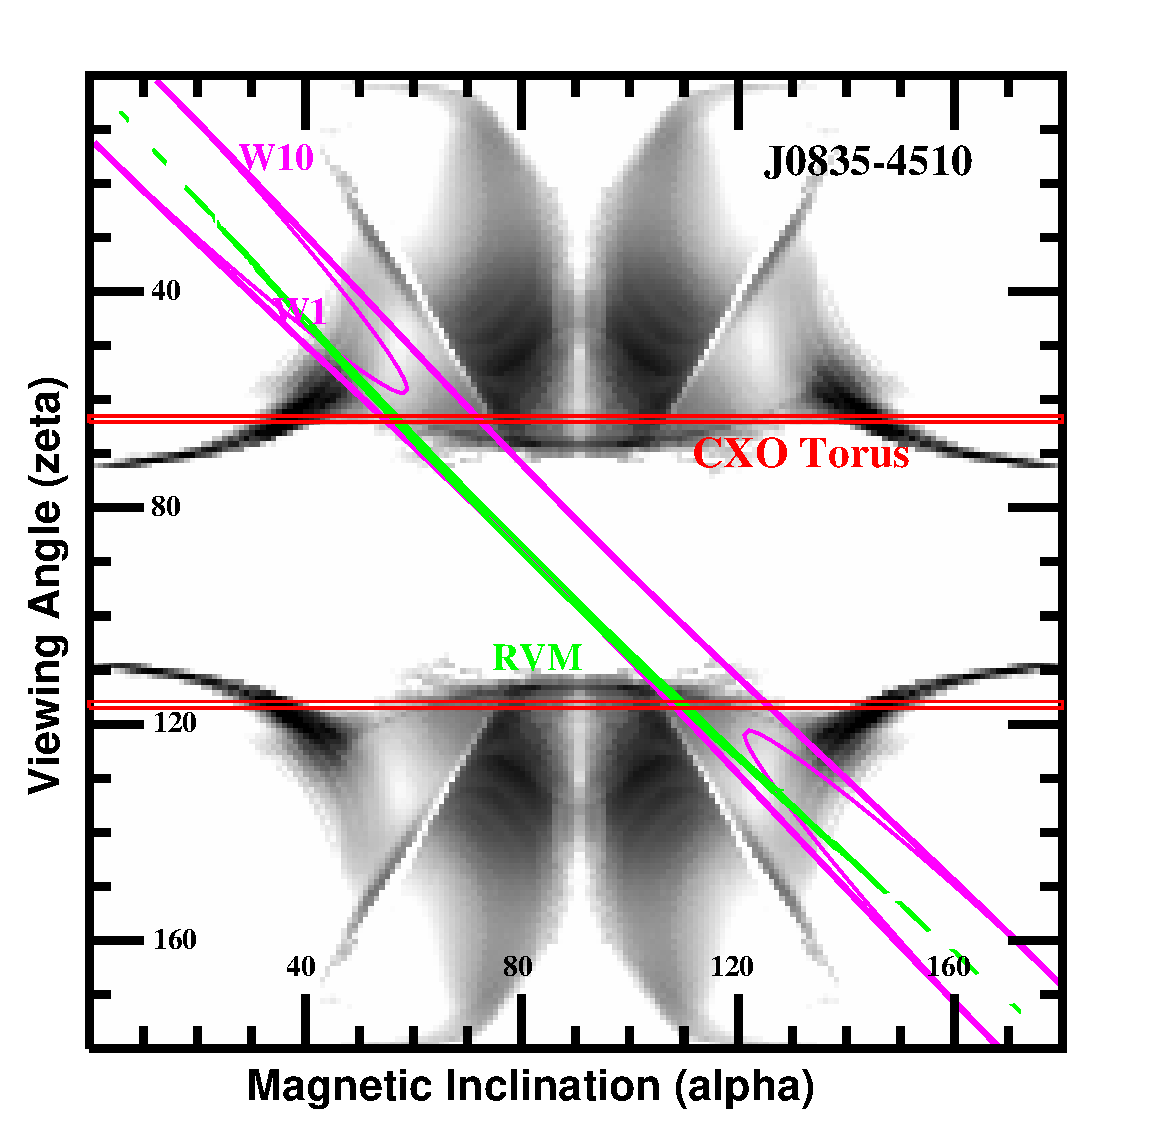
\includegraphics[width=0.5\textwidth]{chapters/multiWaveLength/figures/f2.eps}
\caption[The $\gamma$-ray fit map for Vela in the $\alpha$--$\zeta$ plane with radio polarization, X-ray torus, and pulse width constraints]{
\label{VelaEx} 
Figure taken from \cite{romani2011sub}.
The $\gamma$-ray fit map for Vela in the $\alpha$--$\zeta$ plane with radio polarization, X-ray torus, and pulse width constraints.
The background gray scale shows the goodness of fit of the {\it Fermi} light curve to a
basic outer gap model, with dark colors being better fits. Additionally, red lines mark
constraints from an X-ray pulsar wind nebula torus fit, green contours mark constraints
from RVM, and magenta contours mark constraints from opening angle arguments.
}
\end{center}
\end{figure}


\begin{figure}[htbp]
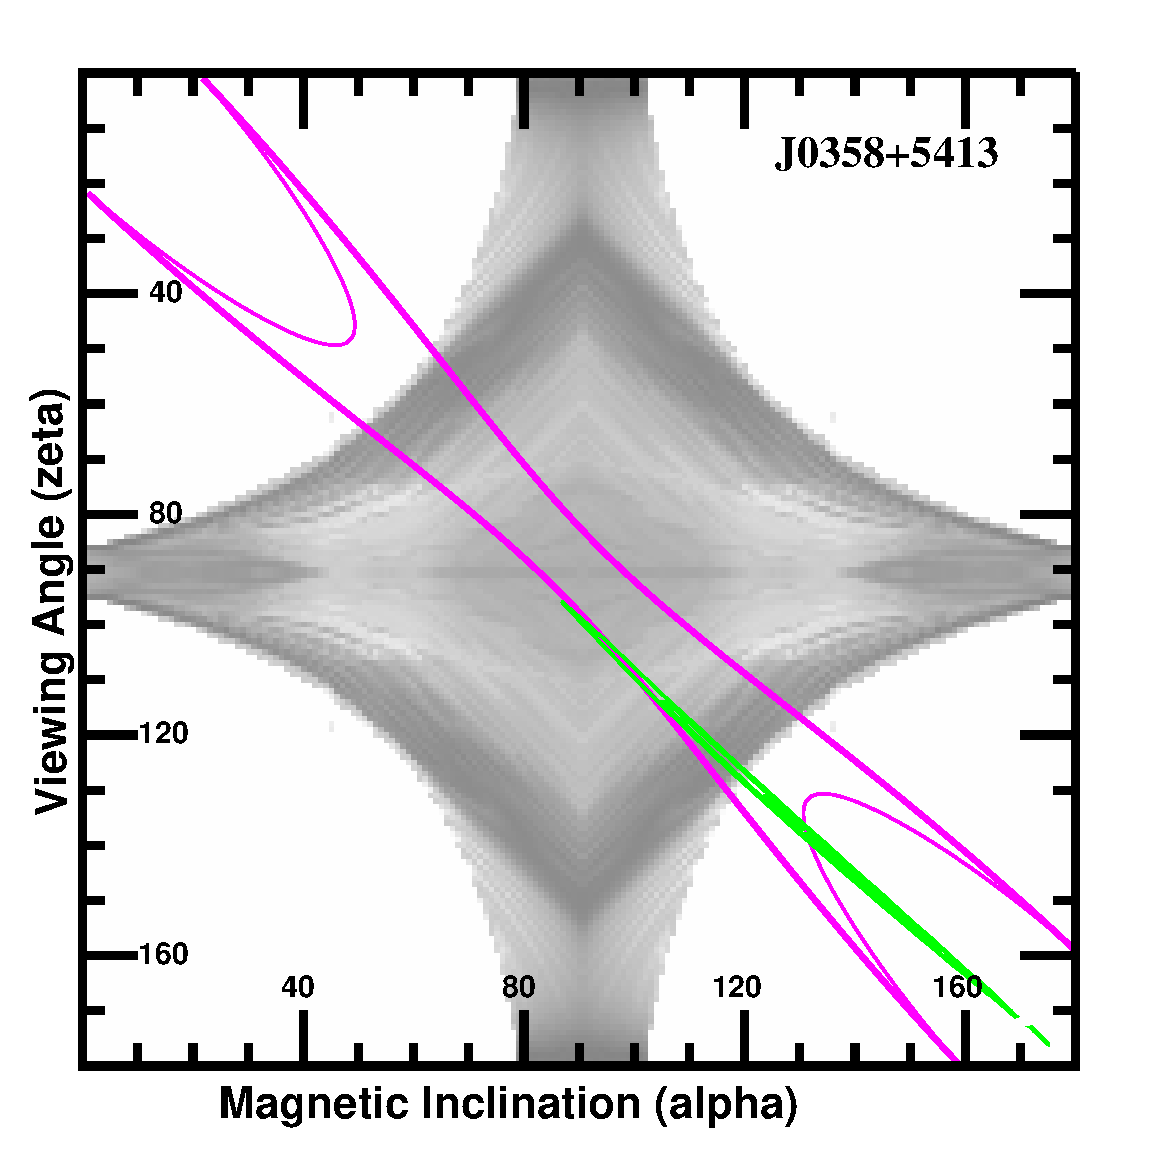
\includegraphics[width=0.5\textwidth]{chapters/multiWaveLength/figures/f3cor_a.eps}
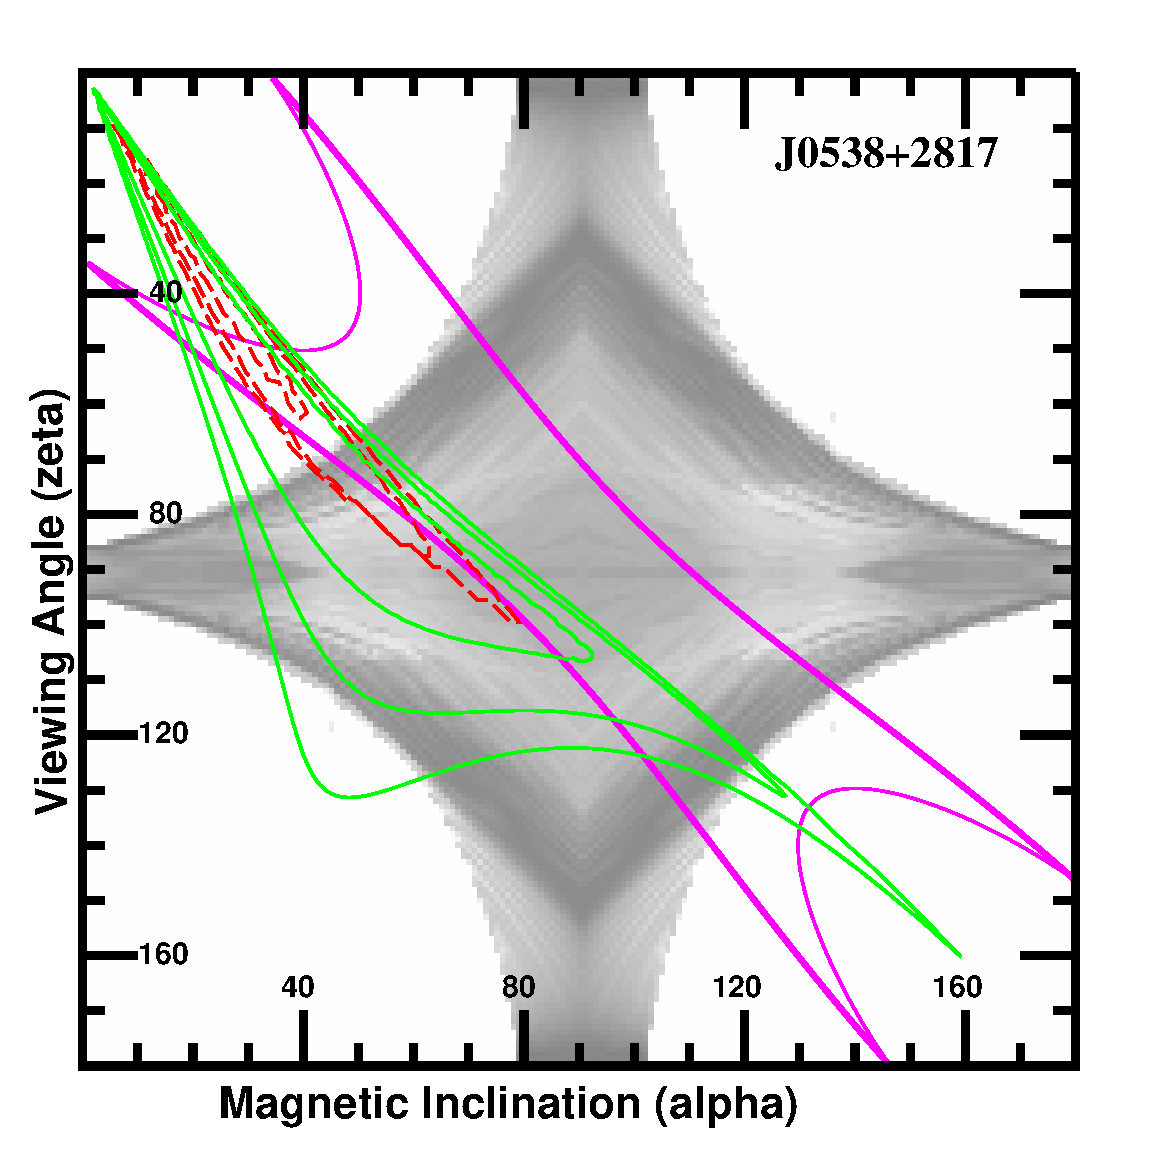
\includegraphics[width=0.5\textwidth]{chapters/multiWaveLength/figures/f3cor_b.eps}
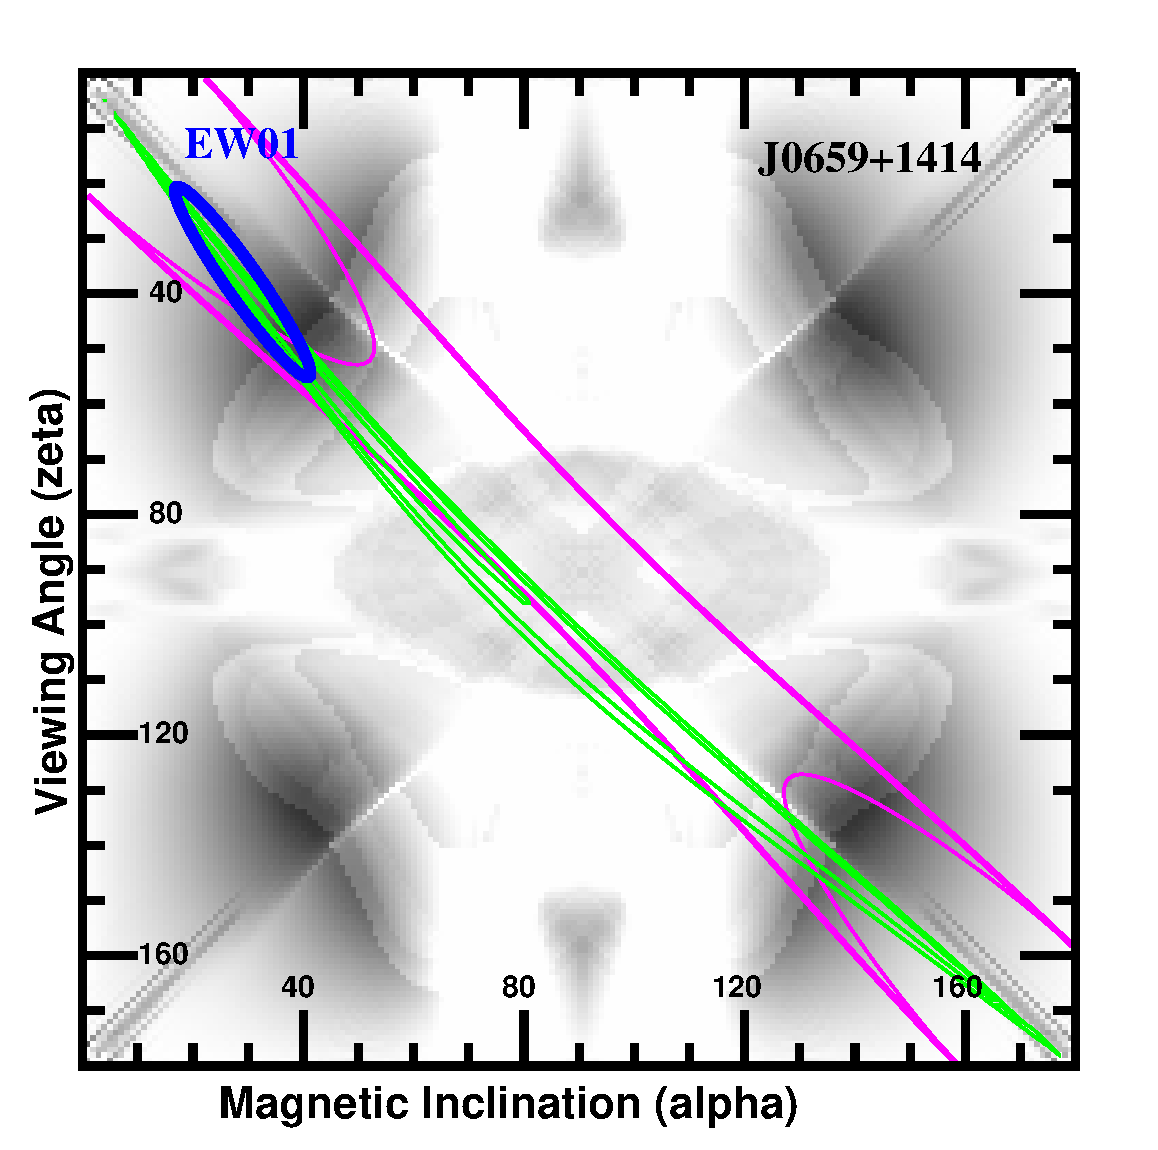
\includegraphics[width=0.5\textwidth]{chapters/multiWaveLength/figures/f3cor_c.eps}
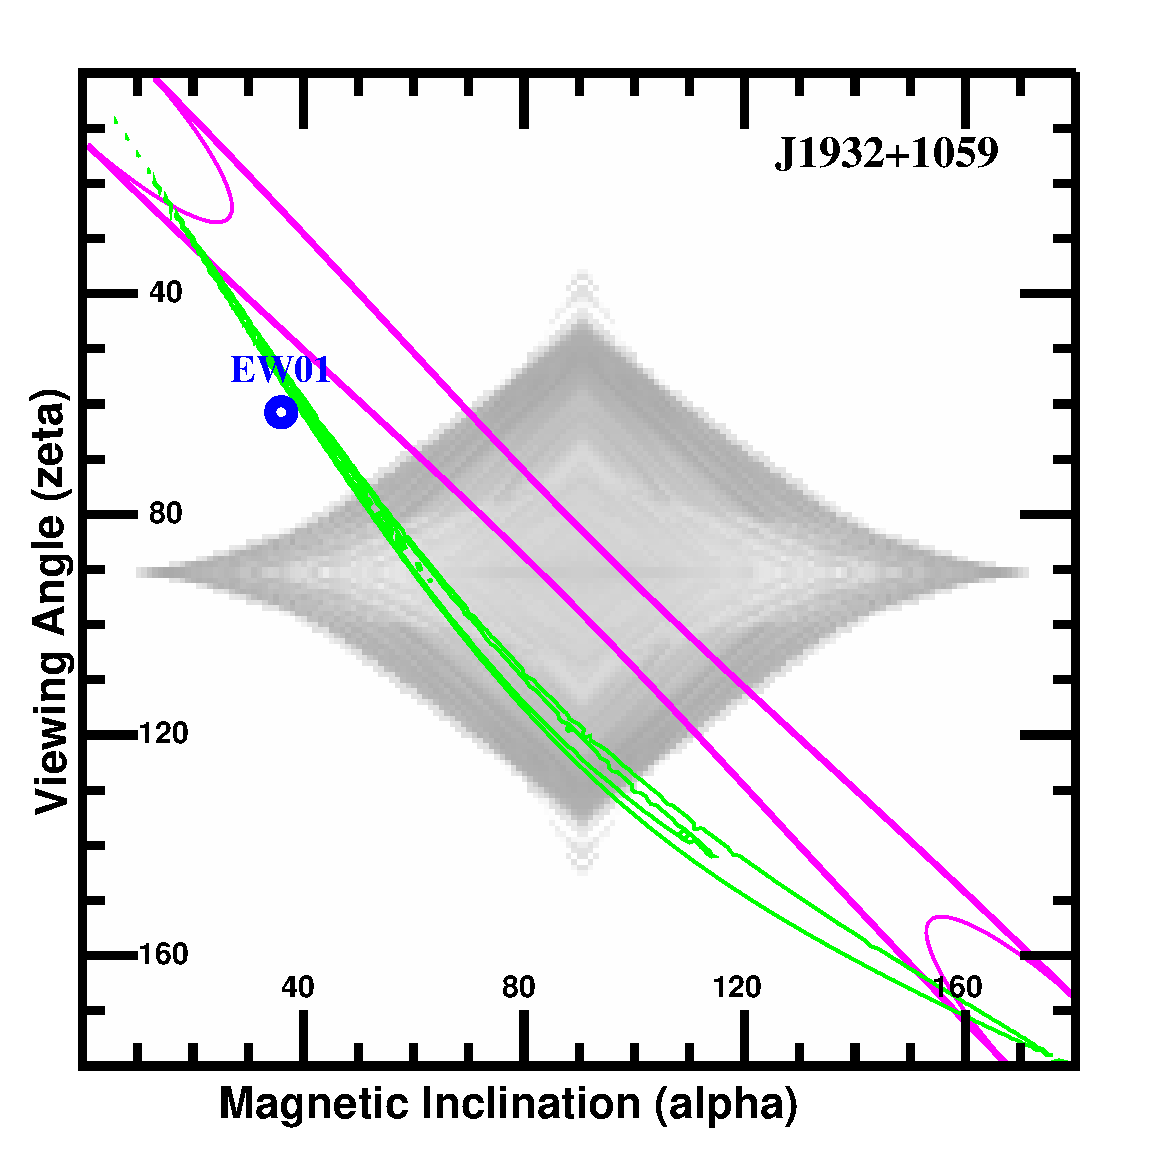
\includegraphics[width=0.5\textwidth]{chapters/multiWaveLength/figures/f3cor_d.eps}
\caption[The $\gamma$-ray fit map for sub-luminous pulsars with parallax
distances in the $\alpha$--$\zeta$ plane with radio polarization and pulse
width constraints]{ \label{plx_const} 
Figure taken from \cite{romani2011sub}.
The $\gamma$-ray fit map for sub-luminous pulsars with parallax 
distances in the $\alpha$--$\zeta$ plane with radio polarization and pulse
width constraints.
The backgrounds show the generic locations providing
sharp outer gap pulses, except for PSR J0659$+$1414, where the background shows the
allowed fits to the observed {\it Fermi} pulses, including lower altitude 
(two-pole caustic model)
%Pole Caustic TPC, Dyks \& Rudak 2003)
emission. 
``Good'' fits here for the other pulsars are in white regions because
of the sub-luminous nature of the pulsars.
Three green contours show the loci of best RVM matches, while the
bold and narrow magenta curves showed the regions allowed by emission from
the static dipole open zone for our estimated emission altitude. For PSR J0659$+$1414 (PSR B0656$+$14)
and PSR J1932$+$1059 (PSR B1929$+$10) the RVM fits of \citet{everett2001emission} are indicated.
For PSR J0538$+$2817 the fits imply large emission altitudes, requiring
a numerical magnetosphere model. The fits to the polarization geometry using
such models are shown by the dashed (red) contours.
}
\end{figure}

\begin{figure}[t!!]
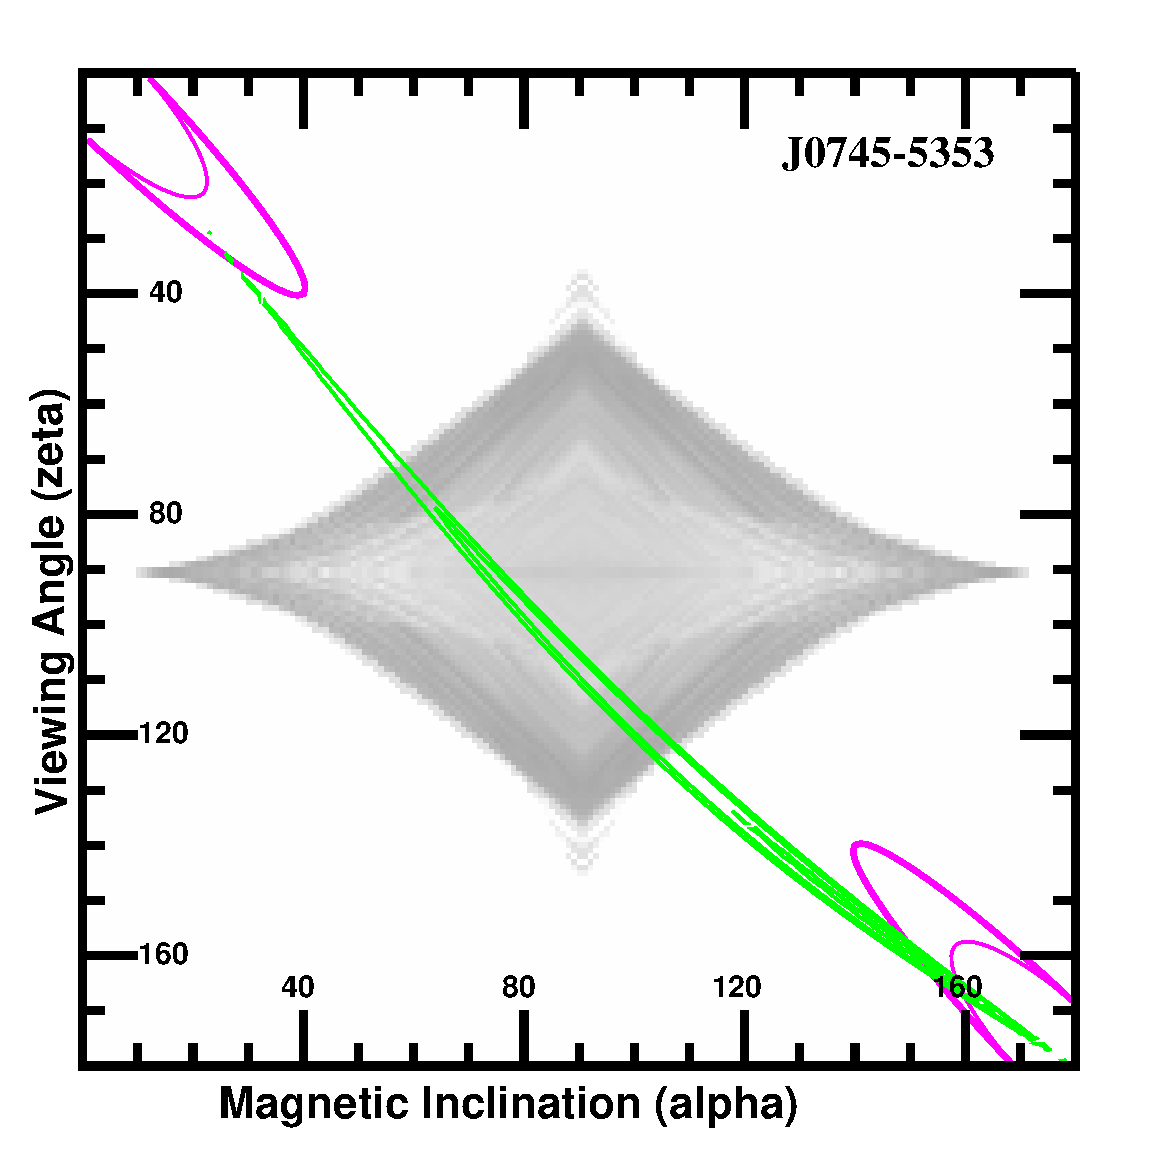
\includegraphics[width=0.5\textwidth]{chapters/multiWaveLength/figures/f4cor_a.eps}
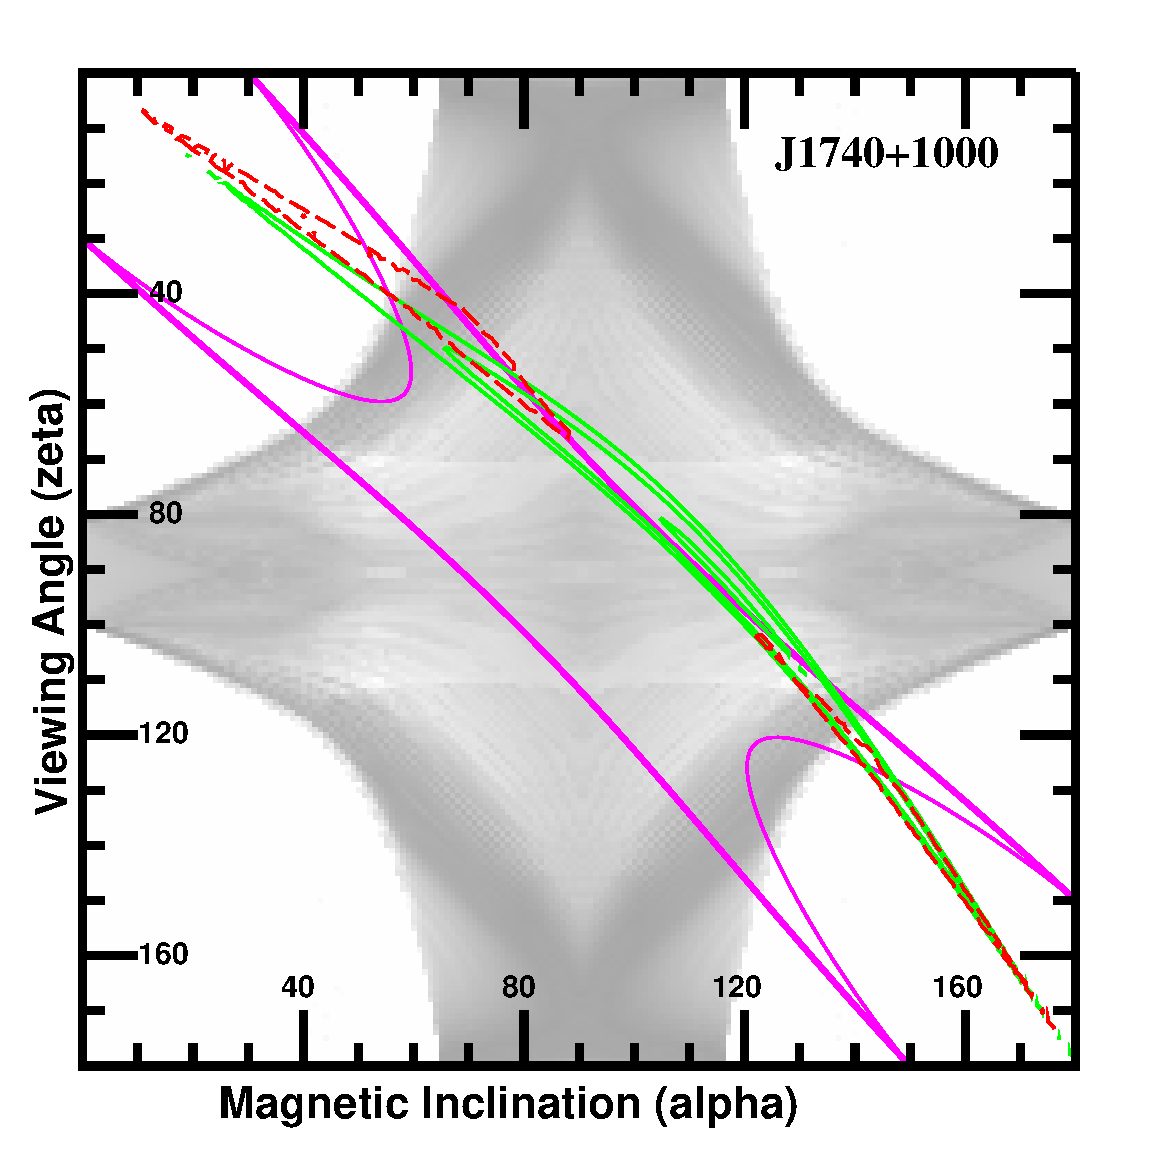
\includegraphics[width=0.5\textwidth]{chapters/multiWaveLength/figures/f4cor_b.eps}
\caption[The $\gamma$-ray fit map for sub-luminous pulsars without parallax 
distances in the $\alpha$--$\zeta$ plane with radio polarization and pulse
width constraints]{\label{noplx_const} 
Figure taken from \cite{romani2011sub}.
The $\gamma$-ray fit map for sub-luminous pulsars without parallax
distances in the $\alpha$--$\zeta$ plane with radio polarization and pulse
width constraints. For geometries
away from the gray background, the sources are not expected to have strong 
outer magnetosphere $\gamma$-ray pulses. 
``Good'' fits here are in white regions because
of the sub-luminous nature of the pulsars.
The PSR J1740$+$1000 data suggest large
emission altitude requiring numerical modeling; the locus of best fits for these models 
is shown by the dashed (red) contours.
}
\end{figure}
Open zone arguments are utilized 
in this paper to constrain acceptable parameter space.  
The parameters $W_1$ and $W_{10}$ represent the
width of the radio pulse assuming that the pulse
ends when the intensity falls below $1\%$ or $10\%$
respectively.  If one definition is more appropriate
for a given pulsar, it will be noted below.
For more details on the relationship between
the phase width and the size of the open zone, 
see Section \ref{sec:beamingGeometry}.

Figure~\ref{VelaEx} is an
example of the use of 
multi-wavelength data to strongly 
constrain the geometry of 
a pulsar.  
The pulsar modeled here is the Vela pulsar (PSR B0833$-$45 or PSR J0835$-$4510).
The pulsar is modeled with $\gamma$-ray data,
radio polarization data, opening angle constraints as
well as X-ray pulsar wind nebula torus fitting 
(see Section \ref{subsec:ToriModeling}).
multi-wavelength data of Vela is used to strongly restricts the possible
parameter space and similar modeling is done for the sub-luminous pulsars.
The magenta contours represent limits
imposed by beaming geometry.  Thin magenta lines represent
$W_{1}$ constant where models with a pulse width
that would accommodate the data are in either corner of the
fitting plane.  For the $W_{10}$ constraint, the models
are limited to those within the thick magenta lines.
The green and red contours show the lowest $\chi^2$ regions
for polarization model fitting.

Unfortunately, none of the other pulsars have clear 
X-ray pulsar wind nebula tori which are strong constraints
on the parameter space.
Four of the pulsars analyzed using polarization have parallax distances available
(PSR J0358$+$5413, PSR J0538$+$2817, PSR J0659$+$1414, and PSR J1932$+$1059) 
and two do not have parallax distances available (PSR J0745$-$5353 and PSR J1740$+$1000).
The fit maps of Figures~\ref{plx_const} and~\ref{noplx_const} show
regions with $\gamma$-ray model gap width of $w\approx L_{\gamma}/\dot{E}$.
The grey background is the fit map of the $\gamma$-ray model to 
a generic single peak pulse except for PSR J0659$+$1414 for which $\gamma$-ray data is
available.  The darker the region, the better the fit.  
Note though that because the pulsars are sub-luminous, the best fit regions
are those that are white regions, since no $\gamma$-rays are present
for these models. 
Blue contours are polarization fit
regions from the literature.  

In the fitting results of PSR J0358$+$5413, the RVM favored $\alpha>110^\circ$.
Additionally, with $W_1$ constraint, $\alpha>130^\circ$ and $\zeta>140^\circ$.
The $W_{10}$ constraints are not more restrictive than the RVM fitting
results.
The pulsar PSR J0358$+$5413 could be sub-luminous but 
some non-sub-luminous geometries are also plausible.

For PSR J0538$+$2817,
the acceptable parameter space given by the
RVM fit is rather large as can be seen in 
Figure~\ref{plx_const}.  However, the combination
of the RVM contours and the $W_{1}$ and $W_{10}$ constraints
are much more restrictive.  With the $W_{1}$ constraint,
the possible models are confined to $\alpha<35^\circ$
and $\zeta<50^\circ$.  The numerical finite-altitude 
fits are included for this pulsar
on the figure in red dashed contours.  These fits
again favor smaller $\alpha$ and $\zeta$ where
one would not expect outer gap emission in $\gamma$-rays.
In contrast, the jet-like feature of the X-ray pulsar
wind nebula does suggest $\zeta\approx90^\circ$
but are too faint to do a formal fit with the torus model
\citep{romani2003pulsar,ng2007origin}.


PSR J0659$+$1414 was previously studied in the radio polarization
\citep{lyne1988shape,everett2001emission,weltevrede2010gamma} 
and the results of \cite{everett2001emission} are included in blue
on the figure.  In our fits to RVM, the model favored $\alpha<80^\circ$
but the pulsar has extended emission well beyond the main peak
such that including the $W_1$ restriction gives $\alpha<35^\circ$.
The goodness of fit given in the figure is for a two-pole caustic
$\gamma$-ray model fit to the {\it Fermi} Large Area Telescope data
available for this pulsar. 
The outer gap model emission best fits are restricted
to $50^\circ<\alpha<130^\circ$ and are well beyond the restrictions
of the strongly extended emission seen in this pulsar.  

The fitting of the polarization data of PSR J1932$+$1059 prefers 
$\alpha<60^\circ$.  However, the additional constraints of 
$W_{10}$ prefers $\alpha<20^\circ$ and $W_{1}$ prefers
$\alpha<15^\circ$.  The RVM fitting contour from
\cite{everett2001emission} is also included on Figure~\ref{plx_const}.
Our analysis would then imply strongly that 
this pulsar is sub-luminous through geometry 
although this pulsar
has a low $\dot{E}$ such that the $\gamma$-ray
emission may have turned off.

PSR J0745$-$5353 does not have a defined parallax distance and
thus can not be definitively categorized as sub-luminous.
From the \cite{cordes2002ne2001} model, the pulsar has a distance
of $0.25$ kpc but a distance of $7.1$ kpc from \cite{taylor1993pulsar}.
The pulsar is sub-luminous if its distance is less than $2$ kpc.
In the combined restriction of RVM and $W_{10}$, $\alpha>150^\circ$
and in the combined restriction of RVM and $W_{1}$, $\alpha>160^\circ$.
Thus if PSR J0745$-$5353 was known to be close enough for detection,
it would be a sub-luminous pulsar.

The pulsar PSR J1740$+$1000 also does not have a parallax distance but
does have a strong dispersion measure distance (Section \ref{sec:interstellarScattering}).  
Both RVM and single-altitude numerical model
fitting was performed on the radio polarization position angle data.
For $W_{10}$ and RVM modeling, $\alpha<70^\circ$ or $\alpha>120^\circ$
is preferred.
For $W_{1}$ and RVM modeling, $\alpha<50^\circ$ or $\alpha>140^\circ$
is preferred.
For $W_{1}$ and single-altitude modeling, $\alpha<30^\circ$ or $\alpha>150^\circ$
is preferred.
So although the pulsar could possibility not be detected due to 
geometry, the parameters are not restrictive enough
to test the model.

In conclusion, this paper attempted to determine whether the non-detection
of these pulsars in the $\gamma$-rays is due to beaming direction
and high altitude emission of the outer gap model.
Although the pulsars all showed evidence of being
sub-luminous due to geometry, none were ruled out
as low-level $\gamma$-ray emitters that will yet be detected
with increased {\it Fermi} Large Area Telescope exposure and pulsed searches.



\section{Conclusions}

In this chapter, several papers are reviewed which take advantage of the 
polarization data to better understand the nature of pulsars.
From the work in these papers, we can see the important role of 
the polarization modeling for radio position angle measurements. 
Both numerical models and RVM were utilized in these studies.
Often times, the rotating vector model is a helpful and easy-to-used model to
interpret
polarization when applied to suitable data.
Additionally, we see the importance of using polarization data in
connection to other wavelengths.
